\documentclass[a4paper,12pt,oneside,openany,table,xcdraw]{article}

\usepackage{setspace}
\usepackage{multirow}
\usepackage{hyperref}
\usepackage{caption}
\usepackage{indentfirst}

\usepackage[brazilian]{babel}
\usepackage[utf8x]{inputenc}
\usepackage{amsmath, graphicx, subfig, enumerate}
\usepackage{float, verbatim}
\usepackage[colorinlistoftodos]{todonotes}
\usepackage{makeidx}
\usepackage{geometry}

\geometry{a4paper, hmargin={3cm, 3cm}, vmargin={3cm, 2cm} }
\setlength{\parindent}{1.0cm}
\graphicspath{{img/}}
\captionsetup{font=small}

\begin{document}
\newcommand{\thedepartment}{Faculdade de Engenharia Elétrica}
\newcommand{\thecourse}{FEELT}
\newcommand{\thetitle}{FONTE LINEAR REGULADA + CIRCUITO AMPLIFICADOR}
\newcommand{\thetype}{Relatório da Disciplina de Eletrônica Analógica I}
\newcommand{\theproftitle}{Bacharel em Engenharia Elétrica}
\newcommand{\thestudent}{Ana Júlia Costa Santana \_ 
11811ETE003\\Lesly Viviane Montúfar Berrios \_ 
11811ETE001}
\newcommand{\theadvisor}{Prof. Daniel Pereira de Carvalho}
\newcommand{\thecity}{Uberlândia}

\thispagestyle{empty}\newcommand*{\themonth}{\ifthenelse{\the\month < 2}{Janeiro }
                  {\ifthenelse{\the\month < 3}{Fevereiro }
                  {\ifthenelse{\the\month < 4}{Março }
                  {\ifthenelse{\the\month < 5}{Abril }
                  {\ifthenelse{\the\month < 6}{Maio }
                  {\ifthenelse{\the\month < 7}{Junho }
                  {\ifthenelse{\the\month < 8}{Julho }
                  {\ifthenelse{\the\month < 9}{Agosto }
                  {\ifthenelse{\the\month < 10}{Setembro }
                  {\ifthenelse{\the\month < 11}{Outubro }
                  {\ifthenelse{\the\month < 12}{Novembro }{Dezembro }}}}}}}}}}}}
                  
\begin{titlepage}
\begin{center}

	\vspace{-0.5cm}

  \begin{figure}[hbt!]
		\begin{center}
		   
\includegraphics[width=2.8cm]{ufu-logo.png}
		\end{center}
	\end{figure}
 	%\vspace{-4cm}

%\begin{doublespacing}

  \Large{\textbf{Universidade Federal de Uberlândia}}\\
  \large{\thedepartment}\\
  \large{\thecourse}\\


\vspace{5.8cm}
  \par
  \large\textbf{\thetitle}
\vspace{5.8cm} 

%\end{doublespacing}
  \par
  \thetype\\
  por\\
  %\hspace{2cm}\large{}\\

\vspace{0.8cm}
\par
  \normalsize{\thestudent}\\ [2cm]
  \theadvisor

\par\vfill
  \thecity, \themonth / \the\year

\end{center}

\end{titlepage}

%% Comeca o documento !

\onehalfspacing
\tableofcontents % sumário
\newpage

\section{Introdução}
Na construcão e planejamento da primeira placa de impresso (\emph{PCB}) está a essência de qualquer curso da Faculdade de Engenharia Elétrica (FEELT), uma vez que, à despeito das dificuldades no entendimento da disciplica teórica, o planejamento e análise da forma de onda da gradezas de tensão e corrente demonstram e ilustram com lucidez cada processo intrínseco do circuito. Nesse sentido, o uso de simuladores, seja \emph{PROTEUS}, \emph{MULTSIM} ou qualquer outro, é ferramenta de imprescindível para a análise do qualquer circuito, e entendimento dos componentes necessários e melhor adaptáveis às exigências do projeto.

O projeto a ser destrinchado em cálculos e demostrações é retirado do material \emph{El Cheapo} \cite{cheapo} cujo título é \emph{Um realmente simples amplificador de potência} (do inglês, \emph{A Really Simple Power Amplifier}). Logo, é preciso planejar a elaboração de dois circuitos: a \emph{fonte de alimentação linear regulada} e o \emph{circuito amplificador}. Sabe-se que o projeto mencionado pode ser substituído em parte por um dispositivo menor (um amplificador operacional), contudo isso não é feito visto que o objetivo principal é o aprendizado dos componentes mais básicos da elétrica: reistores, capacitores, transistores e diodos. %%% indutores representados pelo transformador ??? nunca vi um deles sozinho, só aqueles grandões de exp-ce2.

À respeito da \textbf{\textit{fonte de alimentação linear regulada}}, tratada na Seção \ref{fonte}, pode obter-se melhor experiência, seja na busca por componentes, assim como melhor envolvimento com ferramentas de simulação e elaboração de placas de circuito impresso. Sabendo-se 
 que trata-se de um dispositivo responsável por converter a tensão elétrica alternada em contínua, foi possível verificar experimentalmente as qualidades e resultados de um circuito retificador em ponte, além de filtros capacitivos e circuitos reguladores com diodos zener.

Já o \textbf{\textit{circuito amplificador}}, discutido na Seção \ref{amp}, pode e deve ser realizado com maior empenho, devido à experiência adquirida durante a realização da fonte. Ademais, é interessante sua análise, uma vez que nesse circuito se vê a aplicação de conceitos aprendidos na disciplina teórica, por exemplo de circuitos amplificadores coletor-comum (ou seguidor de emissor) com/sem bootstrapping, amplificadores push-pull, e outros.

Na Seção \ref{fonte}, é descrita o procedimento completo para a construção na fonte, começando pela catalogação dos componentes necessários e seu orçamento, para assim poder estudá-lo em etapas de análise: retificação, filtragem e regulação. Em seguida, na Seção \ref{amp}, são tratadas as peculiaridades do circuito amplificador, o qual abrange trasistores amplificadores de distintas características. Para assim, na Seção \ref{projeto-final} mostrar o resultado final obtido da fonte com o amplificador.

\newpage
\section{Fonte de Alimentação Linear Regulada} \label{fonte}

\subsection{Componentes e orçamento} 
Com intuito de realizar primeiramente o circuito que alimentará o circuito amplificador, ou seja a fonte de alimentação, \emph{El Cheapo} sugere o esquemático da Figura \ref{fonte:esquematico}, o qual já foi adaptado em \cite{cheapo} para componentes mais modernos, por exemplo substituindo os transistores de germânio por outros de silício. Assim, extraí-se os componentes que estão dispostos na Tabela \ref{fonte:componentes}, na qual também verifica-se o orçamento total para esta etapa, nas lojas de eletrônicos de Uberlândia, sendo visitadas Mundo Eletrônico, Ponto Eletrônico, Rádio Peças Uberlândia e Ponto Eletrônico para a aquisição de todos os componentes necessários.
\vspace{0.4cm}

\begin{figure}[H]
\centering
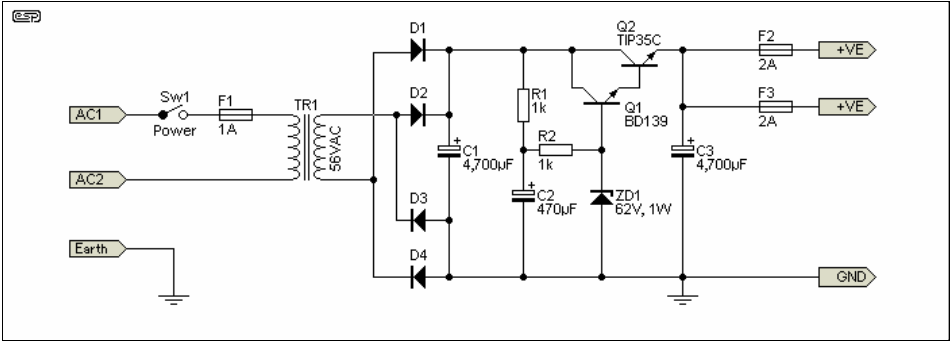
\includegraphics[width=15cm]{fonte-esquematico}
\caption{Esquemático \emph{El Cheapo} do circuito alimentador \cite{cheapo}.}
\label{fonte:esquematico}
\end{figure}
\vspace{0.4cm}

A escolha dos componentes da Tabela \ref{fonte:componentes} também exige análise do circuito mediante um simulador ou análise do circuito, seja por malhas ou nodal, visto que devem ser projetados para uma tensão suficientemente alta. Para todo componente, existe essa limitação intrínseca do material, por exemplo a ponte retificadora escolhida foi a GBJ606, dado que suporta uma corrente máxima de 6A e tensão máxima de 600V.

\begin{table}[H]
\def\arraystretch{1.28}
\centering
\caption{Componentes e orçamento da fonte.}
\label{fonte:componentes}
\resizebox{\textwidth}{!}{%
\begin{tabular}{cc|c|c|c}
\hline
\multicolumn{1}{|c|}{\textbf{Componente}}           & \textbf{Especificação} & \textbf{Quantidade} & \textbf{Preço (R\$)}         & \multicolumn{1}{c|}{\textbf{Descrição}}    \\ \hline
\multicolumn{1}{|c|}{\multirow{2}{*}{Capacitores}}  & $4700 \mu F - 100V$           & 2                   & 35                   & \multicolumn{1}{c|}{C1, C3}                \\ \cline{2-5} 
\multicolumn{1}{|c|}{}                              & $470 \mu F - 100V$            & 1                   & 9,50                  & \multicolumn{1}{c|}{C2}                    \\ \hline
\multicolumn{1}{|c|}{\multirow{2}{*}{Resistores}}   & $1k \Omega$            & 2                   & $ 0,12$        & \multicolumn{1}{c|}{R1, R2}                \\ \cline{2-5} 
\multicolumn{1}{|c|}{}                              & $1k8 \Omega$ - 5W      & 2                   & $4,84$        & \multicolumn{1}{c|}{Descarga do capacitor} \\ \hline
\multicolumn{1}{|c|}{Ponte Retificadora}            & 6A                     & 1                   & 7,15                         & \multicolumn{1}{c|}{Havia a GBJ606}        \\ \hline
\multicolumn{1}{|c|}{\multirow{2}{*}{Transistores}} & BD139                  & 1                   & 0,85                         & \multicolumn{1}{c|}{Q1}                    \\ \cline{2-5} 
\multicolumn{1}{|c|}{}                              & TIP35C                 & 1                   & 5,85                         & \multicolumn{1}{c|}{Q2}                    \\ \hline
\multicolumn{1}{|c|}{Fusível}                       & 4A                     & 1                   & 0,30                         & \multicolumn{1}{c|}{FUS}                   \\ \hline
\multicolumn{1}{|c|}{Borne Painel}                  & 5A                     & 4                   & 	5,25	  & \multicolumn{1}{c|}{Só havia de 20A}       \\ \hline
\multicolumn{1}{|c|}{Placa de fenolite}             & $10\times 15cm$        & 1                   & 6,80                         & \multicolumn{1}{c|}{Tamanho adequado}      \\ \hline
                                                    &                        & \textbf{Total:}     & R\$ 75,66                    &                                            \\ \cline{3-4}
\end{tabular}%
}
\end{table}

\vspace{0.8cm}
\subsection{Estágios do circuito} % com simulações!
Cada componente possui uma função no circuito, que pode ser analisada a nível de tensão e corrente. Espera-se um sinal contínuo na saída, com o qual poderá conectar-se a carga que puxa no máximo 4A (limitação do fusível). Assim, é utilizada uma carga $R_{CARGA}=\dfrac{V_{OUT}}{I_{OUTmax}}=\dfrac{60}{4}=15\Omega$, como observa-se na Figura \ref{fonte:simulacao:circuito} utilizada na simulação.
\vspace{0.6cm}

\begin{figure}[H]
\centering
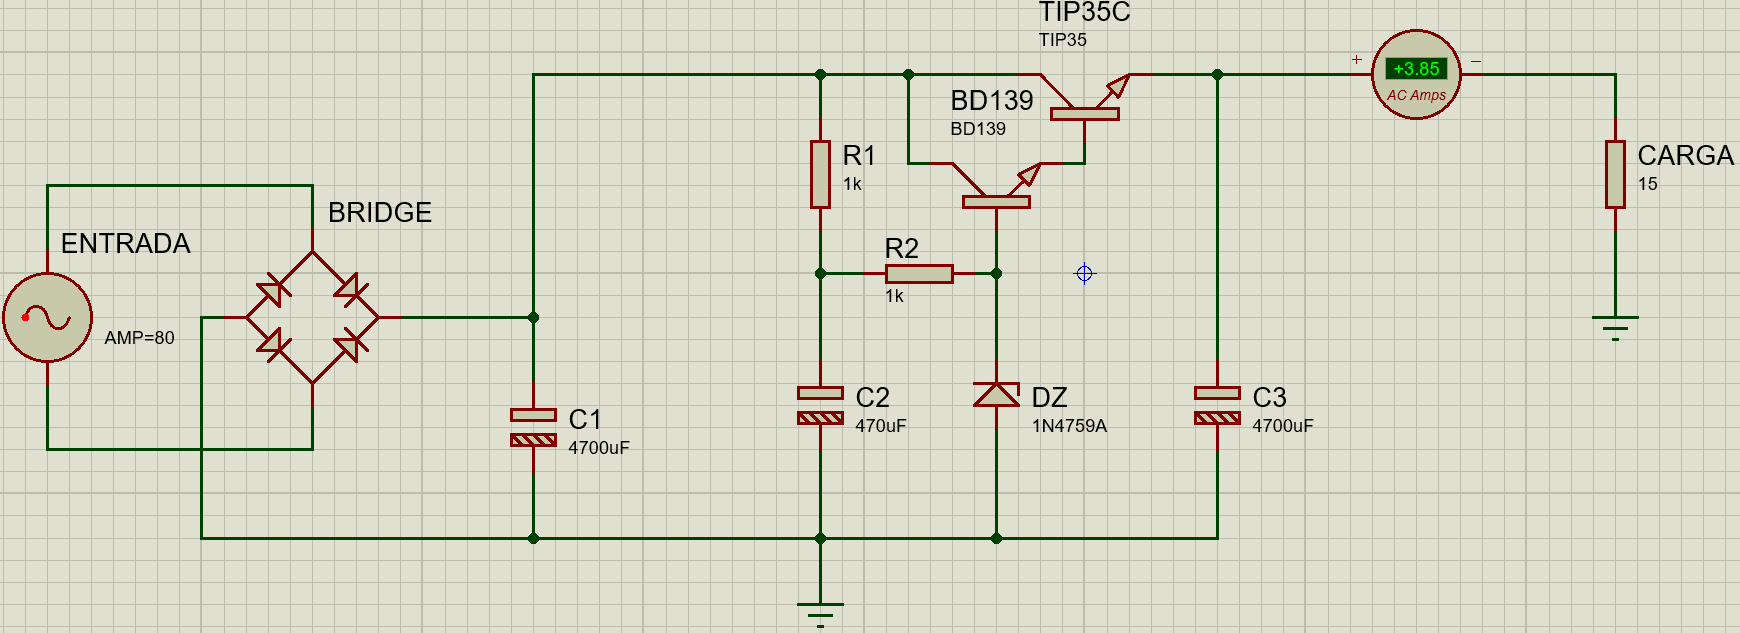
\includegraphics[width=15cm]{fonte-simulacao-circuito}
\caption{Circuito utilizado na simulação da fonte.}
\label{fonte:simulacao:circuito}
\end{figure}
\vspace{0.3cm}

\subsubsection{Retificação}
Esta etapa transforma a tensão alternada em uma tensão contínua pulsante, e é realizada pela ponte retificadora, sendo escolhida a GBJ606 que suporta de 6A, 600 V e atende os parâmetros do circuito montado. Na Figura \ref{fonte:retificacao} observa-se o gráfico da forma de onda da tensão, após a retificação em onda completa pela ponte de diodos.
 
\begin{figure}[H]
\centering
\subfloat[]{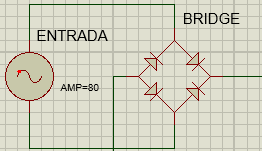
\includegraphics[width=0.47\textwidth]{fonte-retificacao}}\hfill
\subfloat[]{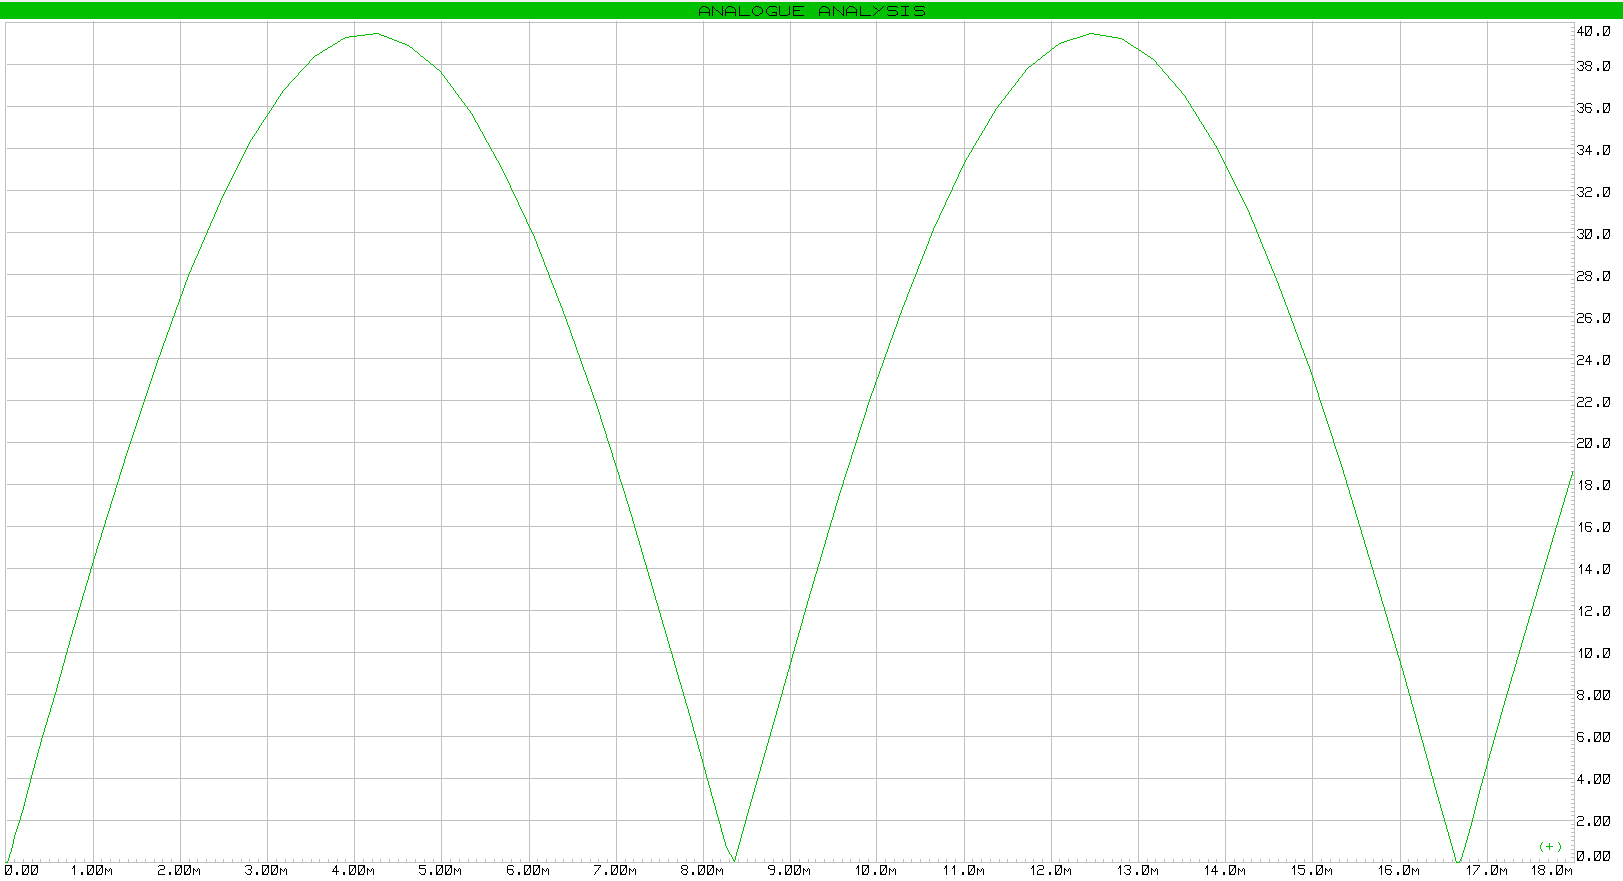
\includegraphics[width=0.5\textwidth]{fonte-retificado}}
\caption{Estágio de retificação (a) circuito (b) resultado da retificação em onda completa.}
\label{fonte:retificacao}
\end{figure}

\vspace{0.2cm}
\subsubsection{Filtragem}
Transforma a tensão contínua pulsante em uma tensão contínua quase perfeita. Mas essa tensão contínua apresenta, quando a fonte é ligada a uma carga, uma oscilação chamada Tensão de Ripple. Essa etapa é realizada pelos capacitores encontrados eno circuito que devido a sua composição, ao sofrer o processo de carga e descarga diminuem a oscilação da tensão já que a tensão fornecida ao circuito agora nos momentos de pulso é suprida pela descarga do capacitor. Porém, como abordado anteriormente, resta ainda o ripple e para eliminar esse fator incômodo pode-se ainda implementar a etapa a de regulação.

\vspace{0.2cm}
\subsubsection{Regulação}
Após a retificação e a filtragem, ocorre a etapa de regulação, com o objetivo de eliminar definitivamente a tensão de oscilação, mesmo com uma carga variável. O diodo utilizado, conta com uma tensão Zener nominal de 62 V para uma corrente de teste de 4 mA.

O comportamento do zener é observado para dois processos, a regulação de linha, que mostra acapacidade da fonte de manter a tensão de saída diante de variações na tensão de entrada.

Se a tensão de entrada aumenta muito, ao invés de ter todo esse acréscimo em cima da carga, o diodo Zener, regula esse valor de tensão, por meio da sua característica de operação em ruptura reversa. Isso é bem observado na corrente, que sofre maiores alterações para que a tensão se mantenha constante.Para o processo inverso, com um descréscimo na tensão de entrada, um processo análogo. As variações na tensão de entrada, são direcionadas ao resistor limitador, mostrando serem válidas as equações abaixo.

\begin{equation}
I_{S}  = I_{Z} +I_{R}  
\end{equation}
\begin{equation}
V_{S}  = V_{in} - V_{Z}
\end{equation}

Existe ainda a  regulação de carga, que mostra a capacidade da fonte de manter uma tensão de saída constante diante de variações na corrente de carga. Que depende da potência requerida pela carga.

\begin{equation}
I_{S}  =\frac{ V_{in} - V_{Z}  }{R_{S}}
\end{equation}

Logo, para toda a variação na corrente de carga é compensada por uma variação oposta na corrente através do diodo Zener, mantendo a tensão constante.
Ademais, releva-se que quando a tensão sobre o diodo zener atinge a tensão de ruptura, o diodo passa a conduzir e se a corrente que passará por ele for suficientemente grande para aumentar sua temperatura, a corrente aumentará 

\vspace{0.2cm}
\subsubsection{Transistores em configuração Darlington}
A configuração Darlington permite maior sensibilidade do transistor, permitindo um ganho $\beta$ ($h_{FE}$) maior. Assim, na Figura \ref{fonte:darlington}, vê-se o par Darlington com os transistores TIP35C \cite{TIP35} e BD139 \cite{BD139}, com $\beta$ associado de $\beta_{total}=25\times 100=2500$.

\vspace{0.2cm}
\begin{figure}[H]
\centering
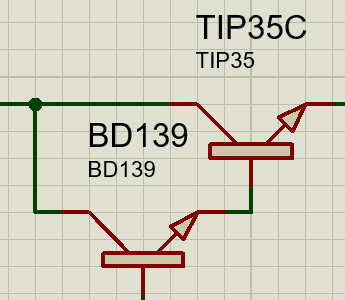
\includegraphics[width=9cm]{fonte-darlington}
\caption{Configuração Darlington na fonte.}
\label{fonte:darlington}
\end{figure}

\subsubsection{Resistor para descarga do capacitor} \label{descarga}
Para segurança do circuito,e daqueles que forem manejá-lo, resistores foram acrescentados em paralelo com os capacitores, para que, ao efetuar o desligamento da placa os capacitores pudessem ser descarregados em segurança.
Para projetar a resistência necessária nos capacitores, as equações conhecidas para descarga num capacitor foram aplicadas.

\begin{equation}
t= RC \cdot ln\bigg( 1 - \frac{V_{C}}{V_{in}} \bigg) 
\end{equation}

Considerndo os capacitores de 4700uF e um tempo de descarga de 10 s, para uma tensão média entre os dois capacitores, $V_{C}$ de $64,85 V$ (de acordo com simulação) e $V_{in}$ de 80 $V_{pp}$, a resitência mínima necessária é de $1,3 k\Omega$, para suprir esses requisitos mínimos, foi utilizado um reistor de $1,8 k\Omega$ de $5W$. 



\vspace{0.3cm}
\subsection{Finalização e considerações sobre a PCB}

\subsubsection{Espessura da linha}
Ao projetar a plca de circuito impresso. Um cuidado maior com relação as trilhas precisa ser tomado, para que não haja problemas quanto a passagem de corrente, e para otimizar a dissipção do calor na placa. 
Para escolher uma espessura de linha que cumprisse tais propósitos, utilizamos o equacionamento de acordo com a norma IPC-2221, que através de sua curva define as constantes k, b e c que são utilizadas no cálculo da espessura da trilha mais adequada.
Iniciando pelo cálculo da área temos:
\begin{equation}
A [\mathit{th^{2}}] = \Bigg(\dfrac{I}{k \cdot (Temp-Rise [deg. C])^{b}}\Bigg)^{\frac{1}{c}}
 \end{equation}
 \vspace{0.3cm}

E em sequência a largura é dada:

\begin{equation}
L [\mathit{th}] = \dfrac{A}{Espessura [oz] \cdot 1,378}
 \end{equation}
\vspace{0.3cm}

Considerando  $k = 0,048$, $b = 0,44$, $c = 0,725$ e a placa de fenolite de \emph{1 OZ}, e uma variação de temperatura de aproximadamente $10^{\circ}C$, descobriu-se um valor para a espessura das linhas de aproximadamente $90 th$, o qual foi utilizado na maioria das trilhas do projeto.

\vspace{0.2cm}
\subsubsection{Projeto final no \emph{PROTEUS}}
Utilizando todos os conceitos já descritos foi possível organizar os componentes em uma placa de cirucito impresso, utilizando o software \emph{PROTEUS}.

\vspace{0.3cm}
\subsection{Análise de testes} %%%%%%%%%%%%%%%%%%%%%%%%%%%%%%%%%%%%%%%%%%%%%%%%% fazer!
Através de testes, ligando a fonte com o auxílio do transformador, logo é possível perceber que a tensão de sída diverge dos 62 V esperados, e isso ocorre porque a placa acaba esquentando bastante devido a sua operação, e assim os diodos que são sensíveis à temperatura acabam operando de um modo não esperado, já que a resistência diminui.


\newpage
\section{Circuito amplificador} \label{amp}
\subsection{Componentes e orçamento} 
O esquemático \emph{El Cheapo}, apresentado na Figura \ref{amp:esquematico}, possui alguns dispositivos que são obsoletos hoje, por exemplo os trasistores de germânio, os quais podem ser equivalentemente substituidos pelos componentes descritos na Tabela \ref{amp:componentes}. 
\vspace{0.2cm}

\begin{figure}[H]
\centering
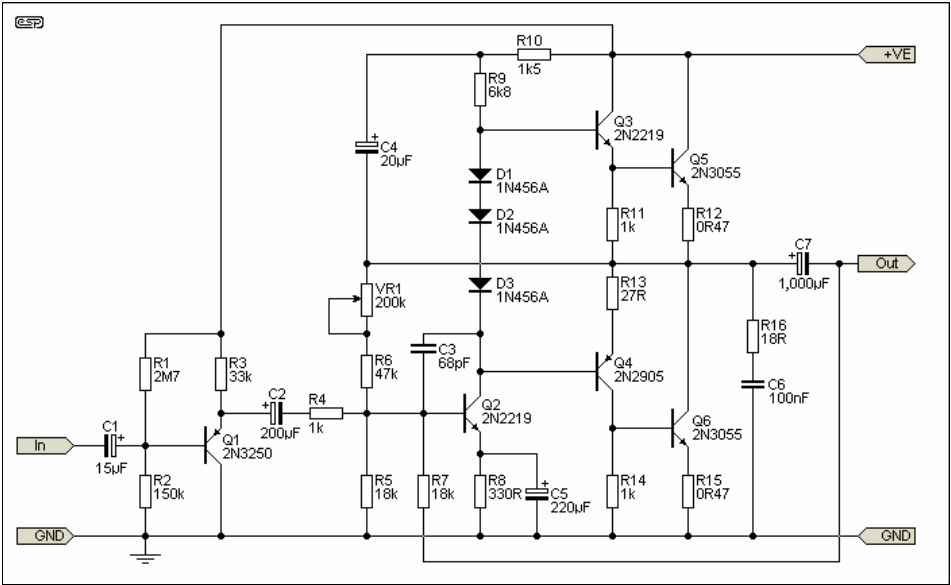
\includegraphics[width=15cm]{amp-esquematico}
\caption{Esquemático \emph{El Cheapo} do circuito amplificador \cite{cheapo}.}
\label{amp:esquematico}
\end{figure}

\vspace{0.4cm}
Dos componentes da Tabela \ref{amp:componentes}, extraídos do esquemático da Figura \ref{amp:esquematico}, ainda são possíveis mudanças para o aprimoramento dos mecanismo do circuito. O capacitor $C7$* por exemplo poderia ter aumento de capacitância para $4700 \mu F$, com o intuito de suprir o amortecimento insuficiente do arranjo de capacitores. %%%%%%%%%%%%%%%%%%%%%%%%%%%%%%%%%%%%%%%%%%%%%%%%%%%%%%%%%%%%%%%%%%%%%%%%%%%%%%%%%%%%%%%%%%%%%%%%%%%%%%%%%%%%%%%%%%%%%%%%%%%%%%%%%%%%%%%%%%%%%%%%%%%%%%%%%%%%%%%%%%%% justificar melhor, entender com graficos e simulacoes
Ademais, é importante ressaltar que os diodos (D1, D2 e D3) devem estar em contato com o dissipador, uma vez que da simulação se terá uma tensão em torno de 4 vezes a tensão de pico da fonte. %%%%%%%%%%%%%%%%%%%%%%%%%%%%%%%%%%%%%%%%%%%%%%%%%%%%%%%%%%%%%%%%%%%%%%%%%%%%%%%%%%%%%%%%%%%%%%%%%%%%%%%%%%%%%%%%%%%%%%%%%%%% explicar falando da tensao, eu acho, por meio de simulacao

\begin{table}[H] \scriptsize
\def\arraystretch{1.28}
\centering
\caption{Componentes e orçamento do circuito amplificador.}
\label{amp:componentes}
\resizebox{\textwidth}{!}{%
\begin{tabular}{cc|c|c|cc}
\hline
\multicolumn{1}{|c|}{\textbf{Componente}} & \textbf{Especificação} & \textbf{Quantidade} & \textbf{Preço} & \multicolumn{1}{c|}{\textbf{Descrição}} & \multicolumn{1}{c|}{\textbf{Observações}} \\ \hline
\multicolumn{1}{|c|}{\multirow{7}{*}{Capacitores}} & $15 \mu F$ & 1 & 0,40 & \multicolumn{1}{c|}{C1} & \multicolumn{1}{c|}{2 cap $10 \mu F$  50V(0,20)} \\ \cline{2-6} 
\multicolumn{1}{|c|}{} & $200 \mu F$ & 1 & 5,00 & \multicolumn{1}{c|}{C2} & \multicolumn{1}{c|}{} \\ \cline{2-6} 
\multicolumn{1}{|c|}{} & $68 p F$ & 1 & 0,50 & \multicolumn{1}{c|}{C3} & \multicolumn{1}{c|}{50V cerâmico} \\ \cline{2-6} 
\multicolumn{1}{|c|}{} & $20 \mu F$ & 1 & 0,76 & \multicolumn{1}{c|}{C4} & \multicolumn{1}{c|}{22UF 100V} \\ \cline{2-6} 
\multicolumn{1}{|c|}{} & $220 \mu F$ & 1 & 6,20 & \multicolumn{1}{c|}{C5} & \multicolumn{1}{c|}{220MF 100V (6,20) 220V (5,00)} \\ \cline{2-6} 
\multicolumn{1}{|c|}{} & $100 nF$ & 1 & 0,42 & \multicolumn{1}{c|}{C6} & \multicolumn{1}{c|}{100k 50V cerâmico} \\ \cline{2-6} 
\multicolumn{1}{|c|}{} & $1000 \mu F$ & 1 & 15,50 & \multicolumn{1}{c|}{C7*} & \multicolumn{1}{c|}{4700MF 63V(15,50)/1000MF 25V} \\ \hline
\multicolumn{1}{|c|}{\multirow{12}{*}{Resistores}} & $2M7 \Omega$ & 1 & 0,09 & \multicolumn{1}{c|}{R1} & \multicolumn{1}{c|}{} \\ \cline{2-6} 
\multicolumn{1}{|c|}{} & $150k \Omega$ & 1 & 0,10 & \multicolumn{1}{c|}{R2} & \multicolumn{1}{c|}{1/8W} \\ \cline{2-6} 
\multicolumn{1}{|c|}{} & $33k \Omega$ & 1 & 0,10 & \multicolumn{1}{c|}{R3} & \multicolumn{1}{c|}{1/8W} \\ \cline{2-6} 
\multicolumn{1}{|c|}{} & $1k \Omega$ & 3 & 0,15 & \multicolumn{1}{c|}{R4, R11, R14} & \multicolumn{1}{c|}{} \\ \cline{2-6} 
\multicolumn{1}{|c|}{} & $18k \Omega$ & 2 & 0,16 & \multicolumn{1}{c|}{R5, R7} & \multicolumn{1}{c|}{1/8W} \\ \cline{2-6} 
\multicolumn{1}{|c|}{} & $47k \Omega$ & 1 & 0,10 & \multicolumn{1}{c|}{R6} & \multicolumn{1}{c|}{1/8W} \\ \cline{2-6} 
\multicolumn{1}{|c|}{} & $330R \Omega$ & 1 & 0,10 & \multicolumn{1}{c|}{R8} & \multicolumn{1}{c|}{1/8W} \\ \cline{2-6} 
\multicolumn{1}{|c|}{} & $6k8 \Omega$ & 1 & 0,10 & \multicolumn{1}{c|}{R9} & \multicolumn{1}{c|}{1/8W} \\ \cline{2-6} 
\multicolumn{1}{|c|}{} & $1k5 \Omega$ & 1 & 0,10 & \multicolumn{1}{c|}{R10} & \multicolumn{1}{c|}{1/8W} \\ \cline{2-6} 
\multicolumn{1}{|c|}{} & $0R47 \Omega$ & 2 & 0,20 & \multicolumn{1}{c|}{R12, R15} & \multicolumn{1}{c|}{1/8W} \\ \cline{2-6} 
\multicolumn{1}{|c|}{} & $27R \Omega$ & 1 & 0,10 & \multicolumn{1}{c|}{R13} & \multicolumn{1}{c|}{1/8W} \\ \cline{2-6} 
\multicolumn{1}{|c|}{} & $18R \Omega$ & 1 & 0,05 & \multicolumn{1}{c|}{R16} & \multicolumn{1}{c|}{1/8W} \\ \hline
\multicolumn{1}{|c|}{Diodos} & 1N456A & 3 & 0,30 & \multicolumn{1}{c|}{D1, D2, D3.} & \multicolumn{1}{c|}{} \\ \hline
\multicolumn{1}{|c|}{\multirow{4}{*}{Transistores}} & BC559 & 1 & 0,93 & \multicolumn{1}{c|}{Q1} & \multicolumn{1}{c|}{} \\ \cline{2-6} 
\multicolumn{1}{|c|}{} & BD139 & 2 & 5,40 & \multicolumn{1}{c|}{Q2, Q3} & \multicolumn{1}{c|}{} \\ \cline{2-6} 
\multicolumn{1}{|c|}{} & BD140 & 1 & 1,68 & \multicolumn{1}{c|}{Q4} & \multicolumn{1}{c|}{} \\ \cline{2-6} 
\multicolumn{1}{|c|}{} & 2N3055 (TIP35C) & 2 & 11,82 & \multicolumn{1}{c|}{Q5, Q6} & \multicolumn{1}{c|}{} \\ \hline
\multicolumn{1}{|c|}{Potenciômetro} & 200k & 1 & 2,75 & \multicolumn{1}{c|}{VR1} & \multicolumn{1}{c|}{} \\ \hline
\multicolumn{1}{|c|}{\multirow{2}{*}{Bornes}} & Painel & 4 & 5,25 & \multicolumn{1}{c|}{} & \multicolumn{1}{c|}{} \\ \cline{2-6} 
\multicolumn{1}{|c|}{} & Jack J2M & 1 & 1,70 & \multicolumn{1}{c|}{} & \multicolumn{1}{c|}{PJ-301} \\ \hline
\multicolumn{1}{l}{} &  & Total: & R\$  59,96 &  &  \\ \cline{3-4}
\end{tabular}%
}
\end{table}

\subsection{Etapas do projeto}
\subsubsection{Primeiro estágio} % Perguntar para o Daniel
\begin{figure}[H]
\centering
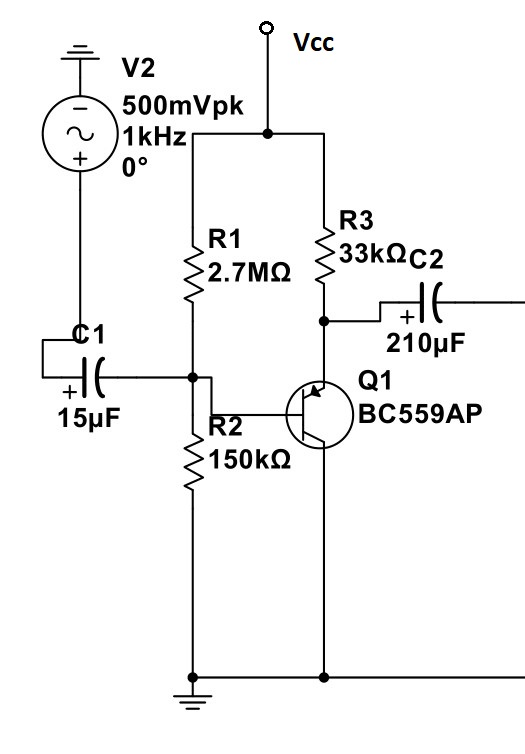
\includegraphics[width=10cm]{multisim-1.jpg}
\caption{Preamp}
\label{multisim-1}
\end{figure}

Dividindo o projeto do amplificador existem 3 estágios. O preampm o driver e o de potência. No inicial para a alimentação do circuito, o trasistor Q1 é utilizado, para parametrizar a entrada no amplificador de potência que conta com uma resistência de 1K, assim o transistor Q1, um seguidor de emissor é utilizado. Dessa forma o estágio de entrada se torna mais estável, o que minimiza os efeitos da Distorção de Intermodulação Transiente.
Realizando alguns cálculos para esta etapa é possível estimar ma tensão de emissor de 4V e uma corrente de coletor de 1,8mA.

\subsubsection{Estágio intermediário}
Neste estágio, conhecido também como driver, o transistor Q2 é usado para realizar uma conversão devido à caractrística inversora do transistor na etapa preamp, mas serve também é utilizado para aumentar o suprimento de corrente, ou seja amplificando-a,possibilitando a excitação  par de transistores de saída. 

Então com o pico máximo positivo na entrada é observada a tensão da fonte no coletor deste transistor, e com o pico mínimo negativo a tensão é zero. 


\subsubsection{Estágio de saída}
No estágio de saída, ou o de potência é utilizado a configuração de pares complementares. Os transistores Q3 e Q4 se encontram acoplados com uma configuração Darlington. Por isso os diodos associados em série são vistos.
Nesta etapa com o uso desse par, cada transistor opera em um ciclo, quesão limitados pelos capacitores. E devido a configuração push- pull eles puxam a energia, logo tendo uma operação como que num sentido de vai e volta.

No final deste etágio, com o auxílio do osciloscópio é possível coletar as formas de onda associadas a entrada e a saída, de forma a tornar possível observar o ganho que o amplificador consegue dar ao sinal de entrada. Para este projeto um ganho de 16 é esperado, porém em testes no laboratório, esta relação ficou em torno dos 15, o que ainda é um valor considerado aceitável, dados os parâmetros de construção.

Abaixo temos o plot das formas de onda coletadas no osciloscópio. Com auxílio de um software matemático, neste caso para a entrada as ponteiras estavam com uma atenuação de 10X:

\begin{figure}[H]
\subfloat[]{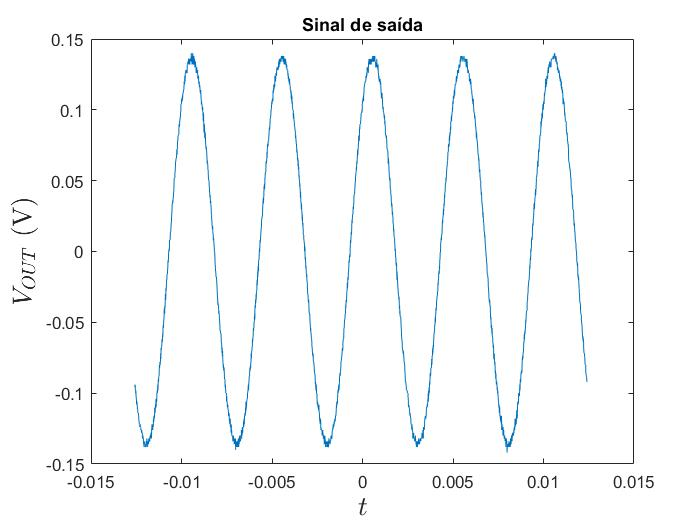
\includegraphics[width=0.47\textwidth]{sinal_saida}}\hfill
\subfloat[]{\includegraphics[width=0.47\textwidth]{ESPECTRO_OUT}}
\caption{Dados de entrada do osciloscóspio.}
\label{ampsuperiorlayout}
\end{figure}

\begin{figure}[H]
\subfloat[]{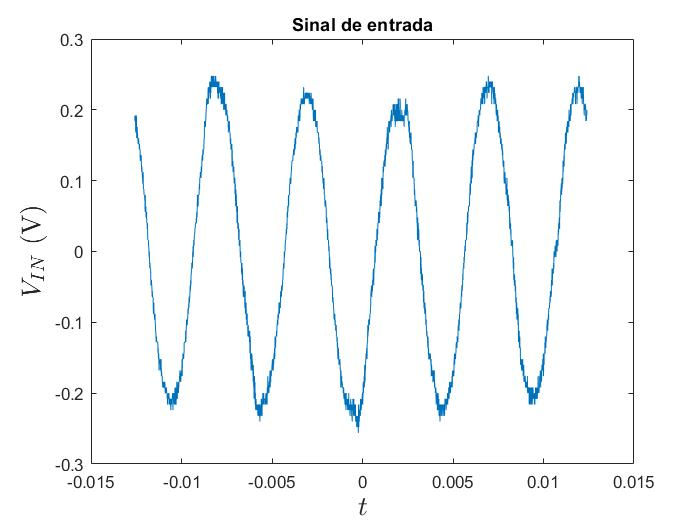
\includegraphics[width=0.47\textwidth]{dados_entrada.jpg}}\hfill
\subfloat[]{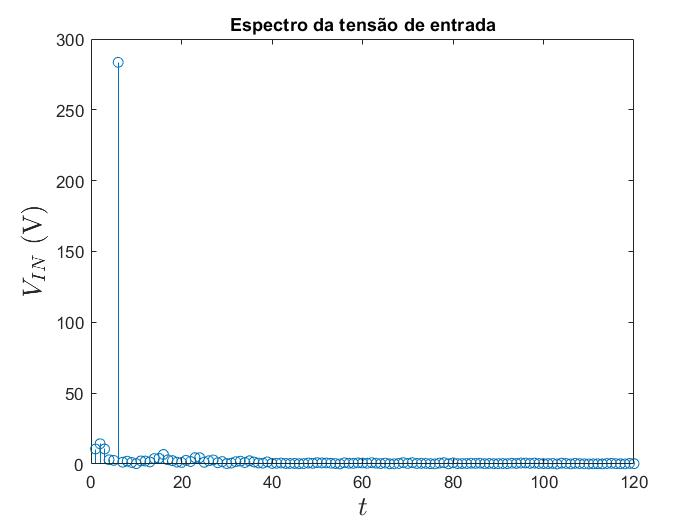
\includegraphics[width=0.47\textwidth]{dados_entrada_espectro.jpg}}
\caption{Dados de saída do osciloscóspio.}
\label{ampsuperiorlayout}
\end{figure}


\subsection{Projeto PCB}
Abaixo seguem os esquemáticos utilizados para a confecção da placas.
Este foi o modelo utilizado para realizar a confecção da placa de circuito impressa. Abaixo, há a disposição dos elementos na placa, assim como a disposição dos mesmos feita no Proteus.

\begin{figure}[H]
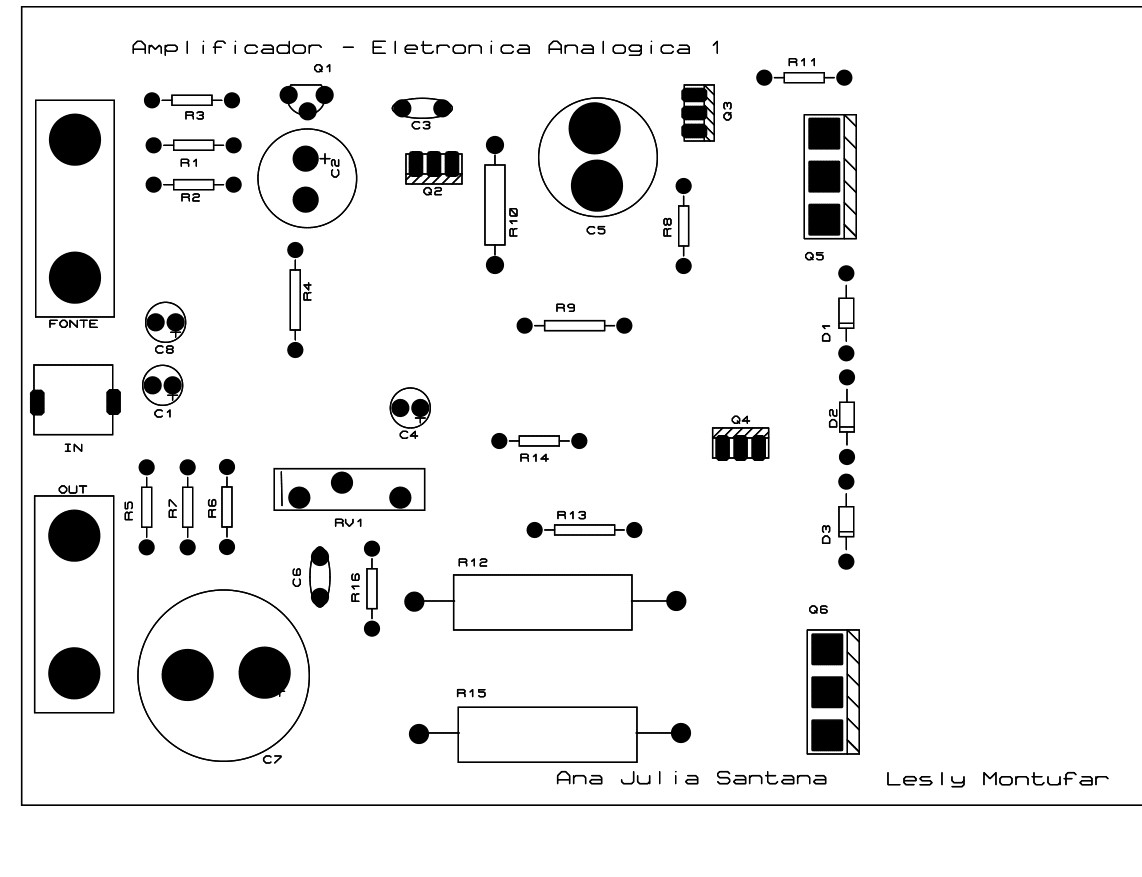
\includegraphics[width=15cm]{ampsuperiorlayout}
\caption{Layout da PCB.}
\label{ampsuperiorlayout}
\end{figure}

\vspace{0.4cm}


\subsubsection{Considerações}
Como o circuito opera em ciclos alternados, o uso de capacitoes cerâmicos se torna mais apelativo, porque estes não possuem polarização fixa como ocorre nos capacitores eletrolíticos, além das alterações que os eletrolíticos tamb~em podem sofrer devido a alta freqência.

No esquemático também dá pra ver um potênciometro sendo utilizado, isso ocorre porque em aplicações onde a resistência necessária precisa ser ajustada atavés de testes práticos, para que seja regulada eficientemente como ocorre neste circuito, o potênciometro é muito mais eficiente, pois é mais fácil realizar ajustes no mesmo do que realizar uma troca constante de resistores fixos.

As resistências de 0,47 nos pares de  transistores acoplados é necessária para que a polariaação dos transistores seja feita de forma mais correta, como resistores de compensação, já que os transistores Darlington são diferentes, sendo eles, um BD139 e o outro BD140, respectivamente Q3 e Q4.

Tratando- se de estabilidade a presença de realimentação no circuito, neste caso do tipo Bootstrap, que é uma realimetação positiva, e auxilia na operação da configuração push-pull, mantendo a tensão AC em ambos os lados do R9 constantes e diminuindo as oscilações que poderiam ser observadas no sinal de saída.
\newpage


\newpage
\section{Conclusões}
\label{projeto-final}
Ao realizar os testes, foi possível ver que a potência máxima alcançada no amplificador projetado, se encontra em torno de 36.44 W, a partir deste ponto, o sinal perde sua regulação e a leitura vista no osciloscópio se torna distorcida. Este acontecimento foi observado ao  elevar a tensão do sinal de entrada em valores maiores que 1.1 Vpp.

Foi fácil perceber que num projeto de tal escala, o planejamento é muito importante, para que não hajam falhas nos resultados,visto que tanto o amplificador quanto a fonte, estão sujeitos a muitoas falhas.

Notou-se que características como a temperatura no ambiente, embora muitas vezes desconsiderada em análises teróricas faz muita diferença na prática, daí a constante necessidade do uso de dissipadores.

Também foi possível observar de uma forma prática tudo o que foi estudado no semestre a respeito de amplificadores, e sua caracterização, sobre as diferenças entre base, coletor e emissor e as relações de ganho no circuito.


\newpage
\begin{thebibliography}{9} 
\bibitem{cheapo}
    Rod Elliott,
    “El Cheapo - A Really Simple Power Amplifier”, ESP, Elliott Sound Products, 2005.
 Disponível em:
 \url{https://sound-au.com/project12a.htm}. Acesso em: out. 2019.
 
 
 % FONTE
 \bibitem{espess}
    Brooks Doug,Graves Dave,
    "Current Carrying Capacity of Vias"
 Disponível em: 
 \url{https://www.ultracad.com/articles/viacurrents.pdf}. Acesso em: out. 2019.
 
 \bibitem{res}
    Soares Camila,
 "Dedução das equações de carga e descarga dos capacitores utilizando equações diferenciais de primeira ordem". 
  Disponível em: 
% \url{https://camilasoares.wordpress.com/2009/04/07/deducao-das-equacoes-de-carga-e-descarga-dos-capacitores-utilizando-equacoes-diferenciais-de-primeira-ordem/}.
https://camilasoares.wordpress.com/2009/04/07/deducao-das-equacoes-de-carga-e-descarga-dos-capacitores-utilizando-equacoes-diferenciais-de-primeira-ordem/ 
Acesso em: out. 2019.
 
 \bibitem{comp}
    Petry Clovis Antonio,
 "D. PROJETO DE PLACAS DE CIRCUITO
IMPRESSO - BÁSICO "
  Disponível em: 
 \url{http://www.professorpetry.com.br/Bases_Dados/Apostilas_Tutoriais/Projeto_PCI_Charles.pdf}. Acesso em: out. 2019.
 
 % AMPLIFICADOR
 \bibitem{amp-classes}
    Eletronics Tutorials,
 "Amplifier Classes"
  Disponível em: 
 \url{https://www.electronics-tutorials.ws/amplifier/amplifier-classes.html}. Acesso em: dez. 2019.
 
 % DATASHEETS
 
 \bibitem{GBJ606} % ponte retificadora
        “6.0A GLASS PASSIVATED BRIDGE RECTIFIER”, DIODES INCORPORATED.
 Disponível em:
 \url{https://www.diodes.com/assets/Datasheets/ds21216.pdf}. Acesso em: out. 2019.
 
  \bibitem{BD139} % transistor
    “BD135/137/139”, FAIRCHILD SEMICONDUCTOR.
 Disponível em:
 \url{http://www.redrok.com/NPN_BD135_45V_1.5A_12.5W_Hfe40_TO-126.pdf}. Acesso em: out. 2019.
 
 \bibitem{TIP35} % transistor
    “Silicon NPN Power Transistors TIP35/35A/35B/35C ”, SavantIC Semiconductor. 
 Disponível em:
 \url{https://pdf1.alldatasheet.com/datasheet-pdf/view/269985/SAVANTIC/TIP35.html}. Acesso em: out. 2019.

\end{thebibliography}
\end{document}
